\section{Anhang}
\subsection{Fattori di conversione e Costanti utili}
\begin{tabular}{@{}llll@{}}
        \toprule
        \textbf{Grandezza} & \textbf{Simbolo} & \textbf{Valore Approssimato} & \textbf{Unità (SI)} \\
        \midrule
        Elettronvolt & $1 \text{ eV}$ & 1.602e-19 & J \\
        Costante di Planck & $h$ & 6.626e-34 & J.s \\
        Velocità della luce & $c$ & 3.0e8 & m/s \\
        Carica elementare & $e$ & 1.602e-19 & C \\
        Massa dell'elettrone & $m_e$ & 9.11e-31 & kg \\
        Costante di Avogadro & $N_A$ & 6.022e23 & mol$^{-1}$ \\
        \bottomrule
\end{tabular}

\subsection{Configurazione elettronica}

Il numero atomico $Z$ indica il numero totali di elettroni che un elemento deve avere.

Ad esempio:

\begin{center}
    Mangan (Mn), Z = 25, \cvt{[Ar]}$\underbrace{\cgn{3}\cbl{d}^\crd{5} \cgn{4}\cbl{s}^\crd{2}}_{e^-\text{di valenza}}$

    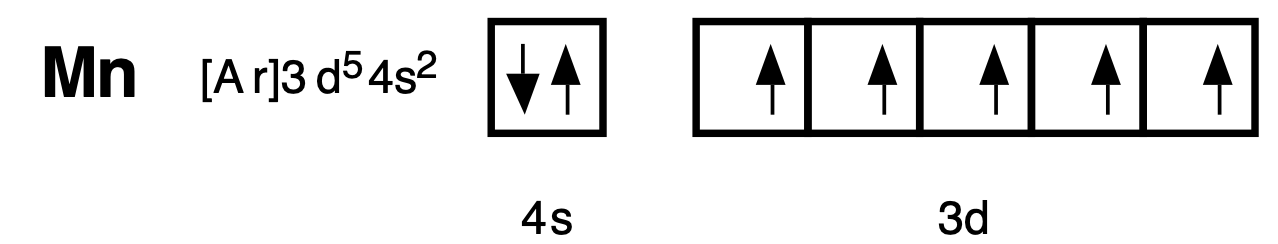
\includegraphics[width=0.5\columnwidth]{Bilder/mangan.png}
\end{center}

\begin{tabular}{cl}
    $\cvt{\blacksquare}$: & I primi 18 $(25-(\crd{5+2}))\ e^-$ sono sistemati come nell'Argon [Ar] \\
    $\cgn{\blacksquare}$: &  Hauptquantenzahl (livello energetico), più il numero è alto più il guscio è lontano\\
    $\cbl{\blacksquare}$: & Bahndrehimpulsq. (sottolivello), vedi \ref{chap:pauli} per il numero di box disponibili\\
    $\crd{\blacksquare}$: & Numero di $e^-$ nel sottolivello
\end{tabular}

\subsection{Formule esercizi}
Dove inserire: Ti consiglio di inserirle come nuovo sottoparagrafo alla fine della Sezione 2.1.1 (Licht come particella: Das Photon)

\renewcommand{\arraystretch}{1.9}
\begin{tabular}{lcl}
    Potenza ottica media & $\bar{P} = \nu_{rep} \cdot E$ & [W] ($\nu_{rep}$ freq. in [Hz], $E$ in [J]) \\ 
    Efficienza del laser & $\eta = \frac{\bar{P}}{P_{ext}}$ & [adimensionale] o [\%] \\ 
    Potenza di picco & $P_{max} = \frac{E}{\tau}$ & [W] ($\tau$ durata dell'impulso in [s]) \\ 
    Intensità max (focalizzata) & $I_{max} = \frac{P_{max}}{\pi \lambda^2}$ & [W/m$^2$] (focale di raggio $\lambda$) \\ 
    Energia del fotone & $E_{phot} = h\nu = \frac{hc}{\lambda}$ & [J] o [eV] \\ 
    \textbf{Fotoni emessi al secondo} & $n_{phot} = \frac{P}{E_{phot}}$ & [s$^{-1}$] \\ 
    \textbf{Corrente generata} & $I = n_{phot} \cdot \eta \cdot e$ & [A]\\
    Tempo andata/ritorno cavità & $t = \frac{2l}{c}$ & [s] ($l$ = lunghezza cavità in [m]) \\ 
    Energia nella cavità & $E_{Kav} = P_{Kav} \cdot t$ & [J] \\ 
    Fotoni immagazzinati & $N_{Kav} = \frac{E_{Kav}}{E_{phot}}$ & [adimensionale] \\ 
\end{tabular}

\textbf{Gruppo 3: Effetto Fotoelettrico}

\begin{tabular}{lcl}
    Lavoro di estrazione & $\Phi = \frac{hc}{\lambda_{max}}$ & [J] o [eV] \\ 
    Flusso di fotoni & $\Gamma_{ph} = \frac{I_{light}}{E_{ph}}$ & [m$^{-2}$s$^{-1}$] ($I_{light}$ in [W/m$^2$]) \\ 
    Densità di fotocorrente max & $J = e \cdot \Gamma_{ph} = \frac{e \cdot I_{light}}{E_{ph}}$ & [A/m$^2$] ($e$ carica elementare) \\ 
\end{tabular}

\textbf{Gruppo 4: Dualismo Onda-Particella (de Broglie)}

Dove inserire: Nella Sezione 2.1.3 (Elektron als Welle: de Broglie Wellenlänge),

\begin{tabular}{lcl}
    Lunghezza di de Broglie ($v$ nota) & $\lambda = \frac{h}{m \cdot v}$ & [m] \\ 
    Lunghezza di de Broglie ($U$ nota) & $\lambda = \frac{h}{\sqrt{2 \cdot m \cdot E_{kin}}} = \frac{h}{\sqrt{2 \cdot m \cdot e \cdot U}}$ & [m] ($U$ tensione in [V]) \\ 
\end{tabular}

\textbf{Gruppo 5: Meccanica Quantistica (Effetto Tunnel)}

Dove inserire: Nella Sezione 2.2.1.2 (Potential mit Höhe V0 und Breite a: Tunnel-Effekt)

\begin{tabular}{lcl}
    Fattore di smorzamento & $\alpha = \frac{\sqrt{2 \cdot m \cdot (V_0 - E)}}{\hbar}$ & [m$^{-1}$] ($V_0$ e $E$ in [J]) \\ 
    Costante di supporto $D$ & $D = \frac{V_0^2}{4 \cdot E \cdot (V_0 - E)}$ & [adimensionale] \\ 
    Probabilità di tunneling & $T = \frac{1}{1 + D \cdot \sinh^2(\alpha \cdot a)}$ & [adimensionale] ($a$ spessore barriera [m]) \\ 
    Definizione $\sinh$ & $\sinh(\alpha \cdot a) = \frac{e^{\alpha \cdot a} - e^{-\alpha \cdot a}}{2}$ & Utile per calcoli esatti \\ 
\end{tabular}